\documentclass[letter, 11pt]{article}
\usepackage[margin=.75in,centering]{geometry}
\usepackage{amsmath}

\usepackage{tikz}
\usepgflibrary{arrows}
\usetikzlibrary{calc,intersections,through,backgrounds}
\usepackage[pdfauthor={Dale Lukas Peterson},
            pdftitle={Feynman Exercises Lecture Challenge},
            pdftex]{hyperref}

\author{Dale Lukas Peterson
\href{mailto:hazelnusse@gmail.com}{$<$hazelnusse@gmail.com$>$}}
\title{\href{http://feynmanlectures.info/announcement.html}{Feynman Exercises
Lecture Challenge}}
\date{\today}

\begin{document}
\pagestyle{empty}
\maketitle

\section*{Restrictions on Solution Method}
In one of the Review lectures Feynman gave to his freshman students, just
before their first big exam, he advised them as follows (copied from Feynman's
Tips on Physics, a problem-solving supplement to The Feynman Lectures on
Physics):

\begin{quote}
  Now, all these things you can feel. You don't have to feel them; you can work
  them out by making diagrams and calculations, but as problems get more and
  more difficult, and as you try to understand nature in more and more
  complicated situations, the more you can guess at, feel, and understand
  without actually calculating, the much better off you are! So that's what you
  should practice doing on the various problems: when you have time somewhere,
  and you're not worried about getting the answer for a quiz or something, look
  the problem over and see if you can understand the way it behaves, roughly,
  when you change some of the numbers.
\end{quote}

The challenge is to solve the problem given below (originally homework for FLP
Vol. I, chapter 23) in the spirit of Feynman's advice, above. It must be solved
without using any calculus or differential equations or integral equations or
difference equations, etc., without iterative numerical methods, nor any such
fancy mathematical tricks! You may use only algebra, geometry, trigonometry,
dimensional analysis, and Newtonian mechanics, in your solution, which should
be guided by your physical intuition (however note: all intuitions used in
solutions must be justified)! Your answer does not have to be exact, but it
should at least be a very close approximation. And be sure to show all your
work! Here is the problem:

\section*{Problem Statement}
The pivot point of a simple pendulum having a natural period of 1.00 second is
moved laterally in a sinusoidal motion with an amplitude 1.00 cm and period
1.10 seconds. With what amplitude should the pendulum bob swing after a steady
motion is attained?

\section*{Solution}
The first step in the solution process is to obtain the equation of motion. To
this end, I introduce a few symbols to represent physical quantities: $m$, $l$,
$g$, being the mass of the pendulum, the length from the pendulum pivot to the
mass center, and the gravitational constant. Without loss of generality, I
assume a simple point mass pendulum with a massless rod, and no dissipation of
any kind.
\begin{figure}[!ht]
  \centering
  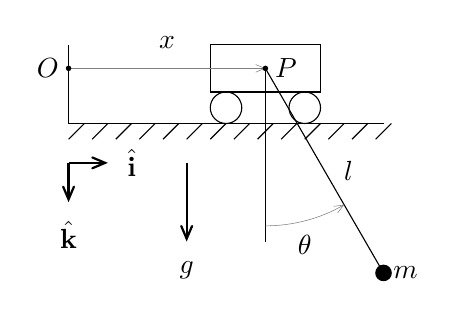
\begin{tikzpicture}[>=angle 45, auto]

    % First draw the ground
    \draw (0, 1) -- (0,0) -- (4,0);
    \foreach \x in {0, .3, ..., 4}
      \draw (\x, -.2) -- (\x+0.2, 0);

    % Next, draw the cart
    \draw (2.0, 0.2) circle (0.2cm);
    \draw (3.0, 0.2) circle (0.2cm);
    \draw (1.8, .4) rectangle (3.2, 1.0);

    % Define a few points
    \coordinate [label=left:{$O$}] (O) at (0.0, .7);
    \coordinate [label=right:{$P$}] (P) at (2.5, .7);
    \coordinate [label=right:{$m$}] (M) at (4.0, -1.898);
    \coordinate (A0) at (2.5, -1.3);
    \coordinate (A1) at (3.5, -1.032);

    % Reference line for theta to be measured from
    \draw[very thin] (P) -- (2.5, -1.5);

    % From inertial origin to pendulum pivot
    \draw[->, very thin, gray] (O) -- (P);

    % Put a solid dot at O and P
    \foreach \point in  {O, P}
      \fill [black] (\point) circle(1pt);

    % Label the displacement at the midpoint of O and P
    \node [label=above:$x$] (X) at ($ (O)!.5!(P) $) {};

    % Draw the mass
    \fill [black] (M) circle(3pt);

    % Draw and label the rod
    \draw (P) -- (M);
    \node [label=right:$l$] (L) at ($ (P)!.5!(M) $) {};

    % Draw and label the arc that indicates the angular displacement
    \draw[->, very thin, gray] (A0) arc (-90:-60:2.0);
    \node [label=below:$\theta$] (T) at ($ (A0)!.5!(A1) $) {};

    % Draw and label the i-j-k unit vectors
    \coordinate (CO) at (0.0, -0.5);
    \coordinate (X) at (0.5, -0.5);
    \coordinate (Y) at (0.0, -1.0);
    \node [label=right:$\hat{\mathbf{i}}$] (I) at (X) {};
    \node [label=below:$\hat{\mathbf{k}}$] (J) at (Y) {};
    \draw[->, thick] (CO) -- (X);
    \draw[->, thick] (CO) -- (Y);

    %Draw and label the direction of the local gravitational field
    \draw[->, thick] ($ (X) + (1.0, 0.) $) -- ++(0, -1.0);
    \node [label=below:$g$] (G) at (1.5, -1.5) {};
  \end{tikzpicture}
  \caption{Pendulum with horizontally translating pivot. $\hat{\mathbf{j}} = \hat{\mathbf{k}} \times \hat{\mathbf{i}}$ points out of
  the page.}
  \label{fig1}
\end{figure}

%Let $O$ be a point fixed in an inertial reference frame $N$.  The position from $O$ to $P$ is
%\[
%\mathbf{r}^{OP} = 0.01\sin\left(\frac{2\pi}{1.1}t\right) \hat{\mathbf{i}}
%\]
%and the acceleration of $P$ relative to the inertial frame $N$ is
%\[
%\mathbf{a}^{P}=
%-0.01\left(\frac{2\pi}{1.1}\right)^2\sin\left(\frac{2\pi}{1.1}t\right)
%\hat{\mathbf{i}}
%\]
The velocity and acceleration of the pendulum mass relative to an inertial
frame are
\begin{align*}
\mathbf{v} &= \dot{x}\hat{\mathbf{i}} + \dot{\theta} \hat{\mathbf{j}} \times \left(l
\sin \theta \hat{\mathbf{i}} + l \cos \theta \hat{\mathbf{k}}\right)\\
&= \left(\dot{x} + l \dot{\theta} \cos \theta \right)\hat{\mathbf{i}} +
\left(-l \dot{\theta} \sin \theta \right) \hat{\mathbf{k}} \\
\mathbf{a} &= (\ddot{x} + l \ddot{\theta} \cos \theta - l \dot{\theta}^2 \sin
\theta) \hat{\mathbf{i}} + (-l \ddot{\theta} \sin \theta - l \dot{\theta}^2
\cos\theta)\hat{\mathbf{k}}
\end{align*}
Two forces act on the mass; the gravitational force $\mathbf{F}_g$ and the force
of the rod $\mathbf{F}_r$:
\[
\mathbf{F}_g = mg\hat{\mathbf{k}} \qquad \mathbf{F}_r = - F \sin \theta
\hat{\mathbf{i}} - F \cos \theta \hat{\mathbf{k}}
\]
where $F$ is a function of time.  Newton's 2nd law yields:
\[
mg\hat{\mathbf{k}} - F \sin \theta \hat{\mathbf{i}} - F \cos \theta
\hat{\mathbf{k}} = m (\ddot{x} + l \ddot{\theta} \cos \theta - l \dot{\theta}^2 \sin
\theta) \hat{\mathbf{i}} + m (-l \ddot{\theta} \sin \theta - l \dot{\theta}^2
\cos\theta)\hat{\mathbf{k}}
\]
Dotting this equation with $\cos\theta\hat{\mathbf{i}} - \sin \theta \hat{\mathbf{k}}$, dividing
through by $ml$ and rearranging, yields:
\[
\ddot{\theta} + \frac{g}{l} \sin \theta =
\frac{0.01}{l}\left(\frac{2\pi}{1.1}\right)^2\sin\left(\frac{2\pi}{1.1}t\right) \cos
\theta
\]
Notice how dotting the Newton's equation into the direction perpendicular to
the rod is a convenient way to eliminate the constraint force
$\mathbf{F}_r$. Linearizing about the downwards position $\theta = 0$, we have
$\sin \theta \approx \theta$ and $\cos \theta \approx 1$, which yields the
following second order linear differential equation:
\[
\ddot{\theta} + \frac{g}{l} \theta =
\frac{0.01}{l}\left(\frac{2\pi}{1.1}\right)^2\sin\left(\frac{2\pi}{1.1}t\right)
\]
Defining $\omega_n^2 = \frac{g}{l}$ and $f_0 =
\frac{0.01}{l}\left(\frac{2\pi}{1.1}\right)^2$, and $\omega = \frac{2\pi}{1.1}$, we can
rewrite the equation of motion as
\[
\ddot{\theta} + \omega_n^2 \theta = f_0 \sin \omega t
\]
Assuming a particular solution of the form $\theta_p(t) =
\Theta\sin\omega t$, differentiating twice with respect
to time, and substituting into the equation of motion yields:
\[
(-\omega^2 + \omega_n^2)\Theta \sin\left(\omega t \right) = f_0 \sin
\omega t
\]
which implies that the amplitude of swing of the pendulum bob after steady
motion is attained is:
\begin{align*}
  \Theta &= \frac{f_0}{\omega_n^2 - \omega^2} \\
         &= \frac{\frac{0.01}{l}\left(\frac{2\pi}{1.1}\right)^2}{(2\pi)^2 -
         (\frac{2\pi}{1.1})^2} \\
         &= \frac{0.047619}{l}
\end{align*}
Where we made use of the fact that the natural frequency is related to the
natural period of oscillation by $\omega_n = 2\pi / T = 2\pi$ rad/s.

Note that this solution depends on the length of the rod.  However, if we
assume Earth's gravitational constant $g=9.81$, then from $g/l=\omega_n^2$ we
can calculate that $l = 0.2485$ m.  Under this assumption, the amplitude of
oscillations is then:
\begin{align*}
  \Theta &= 0.1916 \text{ rad}\\
         &= 10.98  \text{ deg}
\end{align*}
\end{document}
